%Material and methods

\section{Optimal experimental designs}
\begin{formal}
Say how custom designs are more efficient because they fit to the problem rather than having to the change the problem to fit a design.
The main principle in custom design is to maximize an optimality criterion to get the best design possible.
\end{formal}

\subsection{Orthogonal designs}
In design of experiments, orthogonal designs are interesting because they guarantees that each main effect and interaction can 
be estimated independently. Meaning that the effect of one factor or interaction can be estimated separately from the effect of other factors
and that the addition or subtraction of terms in the model does not affect the estimates.
In a regression or ANOVA-type model, the best linear unbiased predictor (or BLUE) of the regression coefficients is obtained by using 
the ordinary least squares (OLS) method, because it minimizes the variance of the estimators. 
These variances are often represented in variance-covariance (VCOV) matrix, 
where the diagonal is the variance of the estimators and the non-diagonal elements are the pairwise covariances between estimators. 
The inverse of this matrix is the information matrix, 
because it summarizes the available information  on the model's coefficients (a low variance means a lot of information, and inversely).
As detailed in \textcite{goos2011optimal}, when the information matrix is diagonal, then the design is said to be orthogonal.

\subsection{Optimality criteria}
In order to generate optimal designs, one needs to use an optimality criterion to compare different designs. 
The two main criteria are the D-optimality and the I-optimality. 
The first one aims at minimizing the variance of the factors effects estimates and is more useful for significance testing. 
D-optimal designs are therefore more appropriate for screening experiments. 
The second one aims at minimizing the average relative prediction variance over the experimental region. 
I-optimal designs are focused on prediction and thus are more suited to response surface experiments.
There also exists a G-optimality criterion that is similar to the I-optimality criterion but minimizes the maximum prediction variance. 
Recent work \parencite{rodriguez2010generating} has shown that I-optimal designs are often better choices than the G-optimal ones. 
Since this is a screening experiment, only the D-optimality is detailed here. 
For more information about I-optimal and G-optimal design, refer to \textcite{goos2011optimal,atkinson2014optimal}.

\subsubsection{D-optimality}
As said previously, for an orthogonal design all the non-diagonal elements of the VCOV matrix are null,
and thus, the determinant is simply the product of all the diagonal elements, i.e. the estimators variances.
Since the goal is to have the smallest variance of the estimates, the VCOV matrix with the smallest determinant will have the 
estimates with the smallest variance. 
Minimizing the determinant of the VCOV matrix is similar to maximizing the determinant of the information matrix. 
Therefore, the design with factor settings that maximize the determinant of information matrix, 
will maximize the available information about the model's parameters. 
This design is called the "D-optimal design", 
where the "D" stands for determinant and the value of the determinant itself is called the "D-optimality criterion".

For any model with two-levels factors and two-factor interaction effects, orthogonal designs will always be D-optimal. 
However if the number of runs is not a multiple of 4 then there are no orthogonal designs available for two-level factors. 
This condition offers little flexibility for experimenters and is not always feasible. 
In contrast, the optimal experimental design approach allows for any number of runs. 
However, in non-orthogonal designs the variance of the estimates is inflated and the estimates are correlated. 
Nevertheless this inflation is usually small and the correlation is too small to cause any concerns.
Therefore there exist non-orthogonal designs that still maximize the information of the model being estimated.
The D-optimal designs may not be unique. For a specified number of runs,
 several designs might have the maximal value for the determinant of the information matrix.\\

%%\paragraph{D-efficiency}
%%The D-efficiency of a given design compares the determinant of the information matrix of that design to an ideal determinant corresponding to an orthogonal design. Since orthogonal design do not always exist, the ideal determinant is defined as $n^p$ for a design with $n$ runs and $p$ parameters in the vector $\boldsymbol{\beta}$.  The D-efficiency is therefore computed as
%%\begin{equation}
%%   \text{D-efficiency} = \left(\dfrac{\vert\mathbf{X}^{\prime}\mathbf{X}\vert}{n^{p}} \right)^{1/p}=
%%    \dfrac{\vert\mathbf{X}^{\prime}\mathbf{X}\vert^{1/p}}{n}
%%    \text{,}
%%\end{equation}
%%where the $p$th root is taken to provide a measure that can be interpreted as a per-parameter measure. The two main problems of the D-efficiency is that it depends on the coding scale of the parameters and that the ideal determinant cannot always be achieved, therefore biasing the measure. The D-efficiency is then only useful to compare design that have the coding for the experimental factors and the same number of runs. For this reason, it is more useful to compare the relative efficiency of two designs
%%it's better to use the relative D-efficiency, defined as
%%\begin{equation}
%%    \text{Relative D-efficiency of Design 1 vs Design 2}=
%%    \left( \dfrac{D_1}{D_2} \right)^{1/p}
%%    \text{.}
%%\end{equation}

%%\subsubsection{I-optimality}
%%\paragraph{Variance of prediction}
%%The variance of the prediction's expectation at the setting $\mathbf{x}$ (a vector of factor levels that corresponds to one of the runs of the design) is 
%%\begin{equation}
%%    var(\Hat{Y}\vert\mathbf{x}) = \sigma_{\epsilon}^2\mathbf{f}^{\prime}(\mathbf{x})(\mathbf{X}^{\prime}\mathbf{X})^{-1}\mathbf{f}(\mathbf{x})
%%    \text{,}
%%\end{equation}
%%where $\mathbf{f}(\mathbf{x})$ is a function that takes a vector of factor settings and expands it to its corresponding model terms. The variance expressed relatively to the error variance $\sigma^2_{\epsilon}$, is
%%\begin{equation}
%%    \text{Relative variance of prediction}=
%%    \dfrac{var(\Hat{Y}\vert\mathbf{x})}{\sigma^2_{\epsilon}}=
%%    \mathbf{f}^{\prime}(\mathbf{x})(\mathbf{X}^{\prime}\mathbf{X})^{-1}\mathbf{f}(\mathbf{x})
%%    \text{.}
%%    \label{eq:relative_var_prediction}
%%\end{equation}
%%Since the prediction's variance depends on the factor settings, $\mathbf{x}$, it is interesting to calculate the averaged variance of prediction over the design space. The average is computed by integrating the relative variance of prediction (\ref{eq:relative_var_prediction}) over the experimental region $\chi$, and dividing it by the volume of the region:
%%\begin{equation}
%%    \text{Average variance}=
%%    \dfrac{\int_{\chi}\mathbf{f}^{\prime}(\mathbf{x})(\mathbf{X}^{\prime}\mathbf{X})^{-1}\mathbf{f}(\mathbf{x}) d\mathbf{x}}
%%    {\int_{\chi}d\mathbf{x}}
%%    \text{.}
%%\end{equation}
%%A design that minimizes the average relative variance of prediction is called a "I-optimal" design. The "I" in "I-optimal" stresses out the fact that an I-optimal design minimizes an integrated variance\footnote{Some authors prefer the term IV-optimal or V-optimal over I-optimal.}.
%%
%%\paragraph{I-efficiency}
%%Similar to the relative D-efficiency, the relative I-efficiency allows for the comparison of two designs in term of average relative variance of prediction. If $P_1$ and $P_2$ are the average relative variance of prediction for two different design, then the relative I-efficiency of the first design to the other is computed as 
%%\begin{equation}
%%    \text{Relative I-efficiency of Design 1 vs Design 2} = 
%%    \dfrac{P_1}{P_2}
%%    \text{.}
%%\end{equation}

\subsection{Generating optimal designs}
In order to generate an optimal design, the determinant of the $\mathbf{X}^{\prime}\mathbf{X}$ matrix needs to be computed multiple times. Therefore algorithms are used to gain time and avoid errors. Several algorithms exist but the most common one is the coordinate exchange algorithm, created by \textcite{meyer1995coordinate}. It has the advantage to run in polynomial time, which means that the time needed to find an optimal design does not explode when the size of the design increases. Another similar algorithm is the point-exchange algorithm, created by \textcite{fedorov2013theory} and modified several times to speed it up \parencite{johnson1983some,atkinson1989construction}. The main drawback of this algorithm is that it needs a list of possible design points as input, which can be quite tedious to do for large designs. In recent years, other types of algorithm such as genetic algorithms \parencite{heredia2003genetic,heredia2004model}, simulating annealing algorithms \parencite{bohachevsky1986generalized,meyer1988constructing} and tabu search algorithms \parencite{jung1996construction} have been used in experimental designs. While these algorithms maintain a level of performance comparable to more traditional design construction techniques, they are not as popular because they are either far more complex, only feasible in some specific cases or better for some specific models and do not lead to designs that make a significant difference in practice.


\subsubsection{Coordinate-exchange algorithm}
The coordinate-exchange algorithm proceeds by iterating through the rows of the matrix of factors settings
\begin{equation}
\mathbf{D}= 
    \begin{bmatrix}
        x_{11} & x_{21} & \ldots & x_{k1} \\
        x_{12} & x_{22} & \ldots & x_{k2} \\
        \vdots & \vdots & \ddots & \vdots \\
        x_{1n} & x_{2n} & \ldots & x_{kn} 
    \end{bmatrix}
    \text{,}
    \label{mat:design_matrix}
\end{equation}
called the design matrix, of an experiment with $n$ runs and $k$ factors. The lines of this matrix essentially represent the coordinates of the runs in the experimental space, where each factor of the experiment is a dimension. This algorithm is called the coordinate-exchange algorithm, because in each iteration of the algorithm, possible changes for every element of the design matrix are considered. \\
It is straightforward to see that the design matrix $\mathbf{D}$ is a submatrix of the model matrix $\mathbf{X}$. It can happen the D-optimality criterion is zero. In those cases, the design is called singular and the inverse of the $\mathbf{X}^{\prime}\mathbf{X}$ matrix does not exist. To avoid singularity, the number of design points (different rows in the design matrix $\mathbf{D}$) must be greater than or equal to the number of model parameters.\\

The algorithm starts by generating a random design. For all continuous factors, the algorithm generates random values on the interval $[-1,+1]$. For all factors that are categorical, the algorithm randomly chooses a value in a discrete set of levels. This random starting design is almost always non-singular. If the design happens to be singular, then another new random starting design is computed.\\
In the next step, the algorithm improves the design on an element-by-element basis. For each element of the starting design, $x_{ij}$, a change to either $-1$ or $+1$ is considered, and its impact on the D-optimality criterion is evaluated. The change that increases the value of the D-optimality criterion the most, is kept. After investigating changes in each element of the design, the process is repeated until no element changes within an entire iteration through the factor settings or until a prespecified maximum number of iterations is reached. The obtained design is the best among a set of neighbouring designs but it is often a locally optimal design that is different for each random starting design. To select the best among all locally optimal designs, the algorithm is repeated a large number of times. The globally optimal design is then selected among all the locally optimal ones, as the one that yields the highest D-optimality criterion.

\subsection{Generating the design}
A custom design was created for the experimental set-up of the phenotyping platform, where the goal was to quantify the genotype and tank effect. Four factors were considered:

\begin{description}[align=left]
\item [Tank] In which tank was the plant situated (moving or still).
\item [Strip] Which of the 99 strip was used (1 to 99).
\item [Position] What was the position on the strip (1 to 5).
\item [Genotype] Which one of the 30 genotypes was used (1 to 30).
\end{description}

To fit the design, the design of experiment (DOE) tool was used in JMP. The four categorical factors were specified and \textit{Tank} and \textit{Strip} were set to "very hard to change" and "hard to change", respectively. Two whole plots of 99 sub-plots each were specified to match the tanks and the strips. With 99 strips of five positions inside two tanks, 990 experimental runs were available.\\
Initially the design was supposed to take into account the 99 different strips individually but the program couldn't converge to an optimal design because of its complexity. Instead only 33 strips were considered and the design was replicated 3 times to match the number of runs. Figures \ref{fig:moving_layout_30_geno} and \ref{fig:still_layout_30_geno}, display a schematic view of the design for the moving and still tank respectively.\\
The seeds were provided by the national institute of agronomic research (INRA) in Montpellier, France, as part of their own research on these historical series\footnote{Historical series correspond to varieties that have been cultivated and bred for some time, mainly due to their physiological specificities.}. They sent a total of 30 seeds per genotype and besides that, an extra 150 seeds of another genotype, called the "border genotype", was sent by the provider. The main utility of the border genotype is to fill the gaps left by non germinated seeds. Since, in this experiment, only 900 runs (30 genotypes x 30 seeds) were occupied, the border genotype was also be used to fill the 90 empty runs. Since this genotype is not part of the historical series, it was not considered in the design of the experiment.

\begin{sidewaysfigure}[ht]
    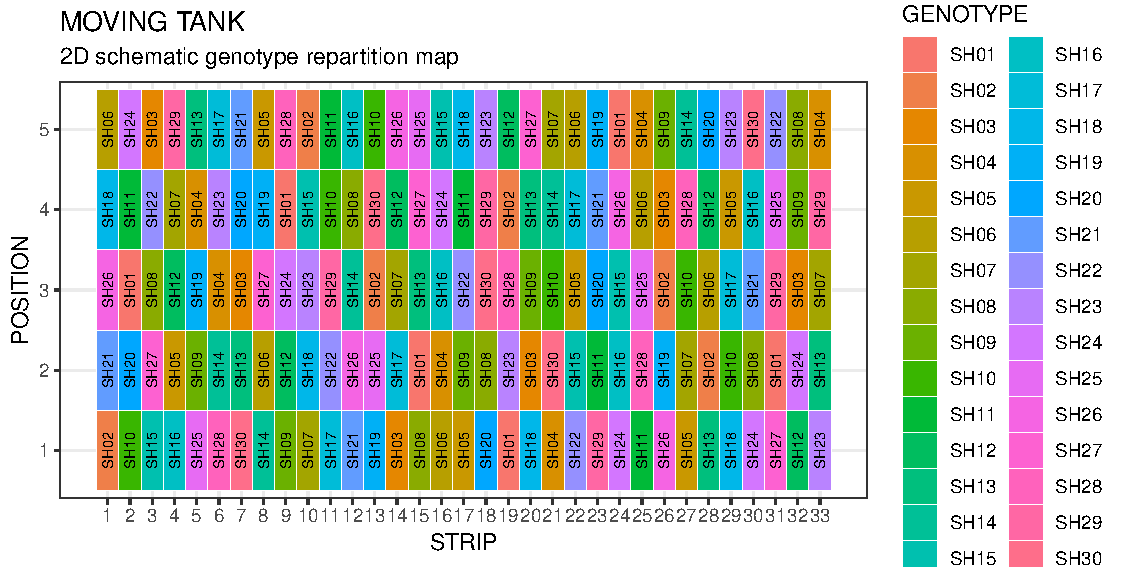
\includegraphics[width=\textwidth]{figures/moving_layout_30_genotypes.pdf} 
    \caption{2D schematic representation of the experimental design for 33 individual strips and 30 genotypes in the moving tank.}
    \label{fig:moving_layout_30_geno}
\end{sidewaysfigure}

\begin{sidewaysfigure}[ht]
    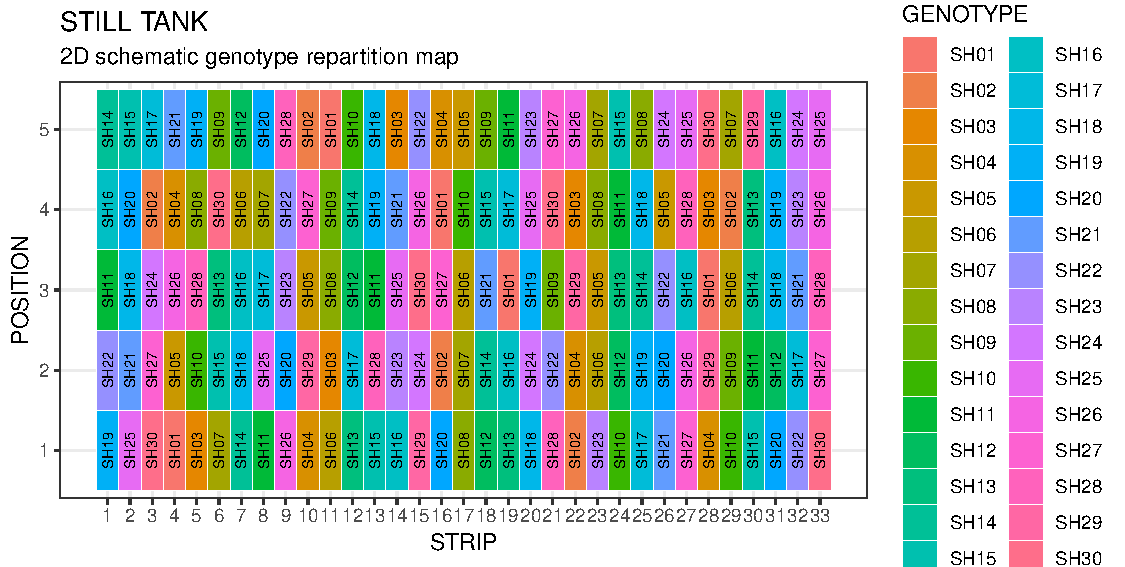
\includegraphics[width=\textwidth]{figures/still_layout_30_genotypes.pdf} 
    \caption{2D schematic representation of the experimental design for 33 individual strips and 30 genotypes in the still tank.}
    \label{fig:still_layout_30_geno}
\end{sidewaysfigure}

\subsection{Design's characteristics}


\section{Phenotyping experiment}
The phenotyping experiment took place between February 25th and March 13th. The seeds were first germinated and then transferred onto the platform. After the end of the experiment the plants were weighted, dried and weighted again to obtain dry and fresh weight.

\subsection{Germination}
Previous experiments in the greenhouses showed that germination of maize seeds on the platform often lead to asphyxiation of the seeds. 
Because of this, the seeds were germinated in an outside germination chamber and were only transferred onto the platform once germinated.

%%A previous germination experiment was conducted in the greenhouse, in a smaller version of the phenotyping platform, to compare seed germination in different type of substrate. In this experiment, 60 maize seeds were set on 6 strips of 5 positions in 2 small reproductions of the aeroponic tanks of the platform. In each tank, a different kind of cork was used to see which one allowed a better germination. It showed that germination rates were fairly low (around 6\%) for both type of cork, mainly because the seeds were asphyxiated in the corks. This lead to the choice of an outside germination to avoid low germination and seed asphyxiation problems.\\
%%The seeds were germinated in a germination chamber outside of the platform and were transferred onto the platform once they were germinated.

The seeds were placed in a temperature-controlled room at 20$^{\circ}$C for 3 days, inside a germination chamber. The chamber consisted of 2 PVC trays to which an air-fog machine was connected, to keep the seeds moist. 
Inside each tray, PVC plates were disposed diagonally and evenly spaced (fig. \ref{fig:germination_chamber_diagram}). On those plates, the seeds were arranged on a filtering paper sheet with ledges to support the weight of the seeds (figure \ref{fig:germiantion_ledge} and figure \ref{fig:photo_germination_plate}). The bottom of the trays was filled with water to keep the filtering paper moist. 
There were 17 plates in total, 15 for the 30 genotypes and 2 for the border genotype (150 seeds dispatched on 2 plates). 

    \begin{figure}[!htb]
        \centering
        \begin{subfigure}[b]{0.95\textwidth}
            \centering
            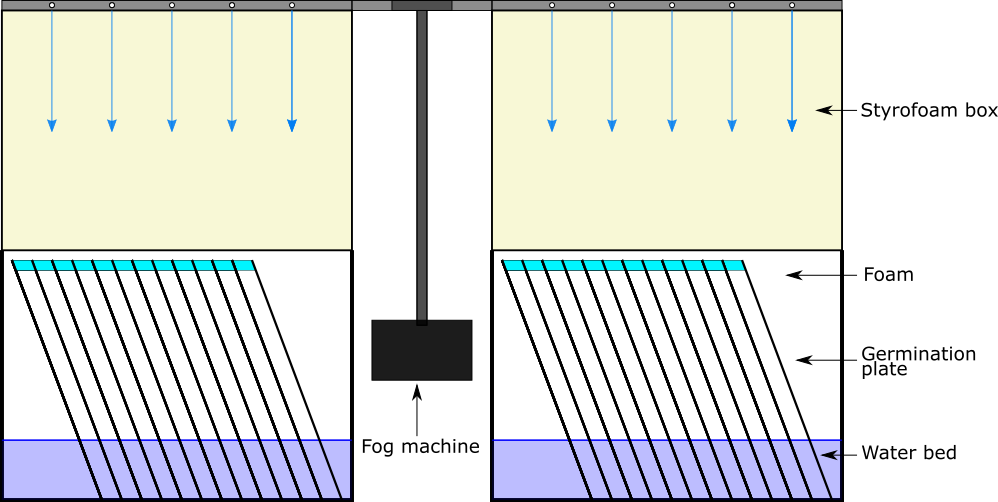
\includegraphics[width=\textwidth]{figures/germination_chamber_diagram.png}
            \caption[]%
            {Global schematic view of the germination chamber: a fog machine assure constant humidity in the germination chambers by creating fog at regular intervals (the blue arrows represent the path of the fog). The plates are placed at a 60$^{\circ}$ angle and 5 cm apart}    
            \label{fig:germination_chamber_diagram}
        \end{subfigure}
        \vskip\baselineskip
        \begin{subfigure}[b]{0.475\textwidth}   
            \centering 
            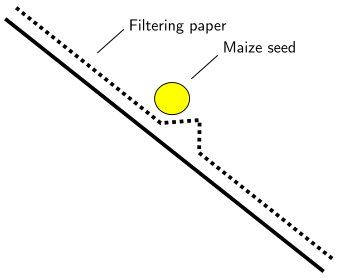
\includegraphics[width=\textwidth]{figures/germination_ledge.png}
            \caption[]%
            {Schematic view of a germination ledge on a PVC plate: each seed is fixed in position on the ledge by an additional drop of agar solution to avoid any fall-off}    
            \label{fig:germiantion_ledge}
        \end{subfigure}
        \quad
        \begin{subfigure}[b]{0.475\textwidth}   
            \centering 
            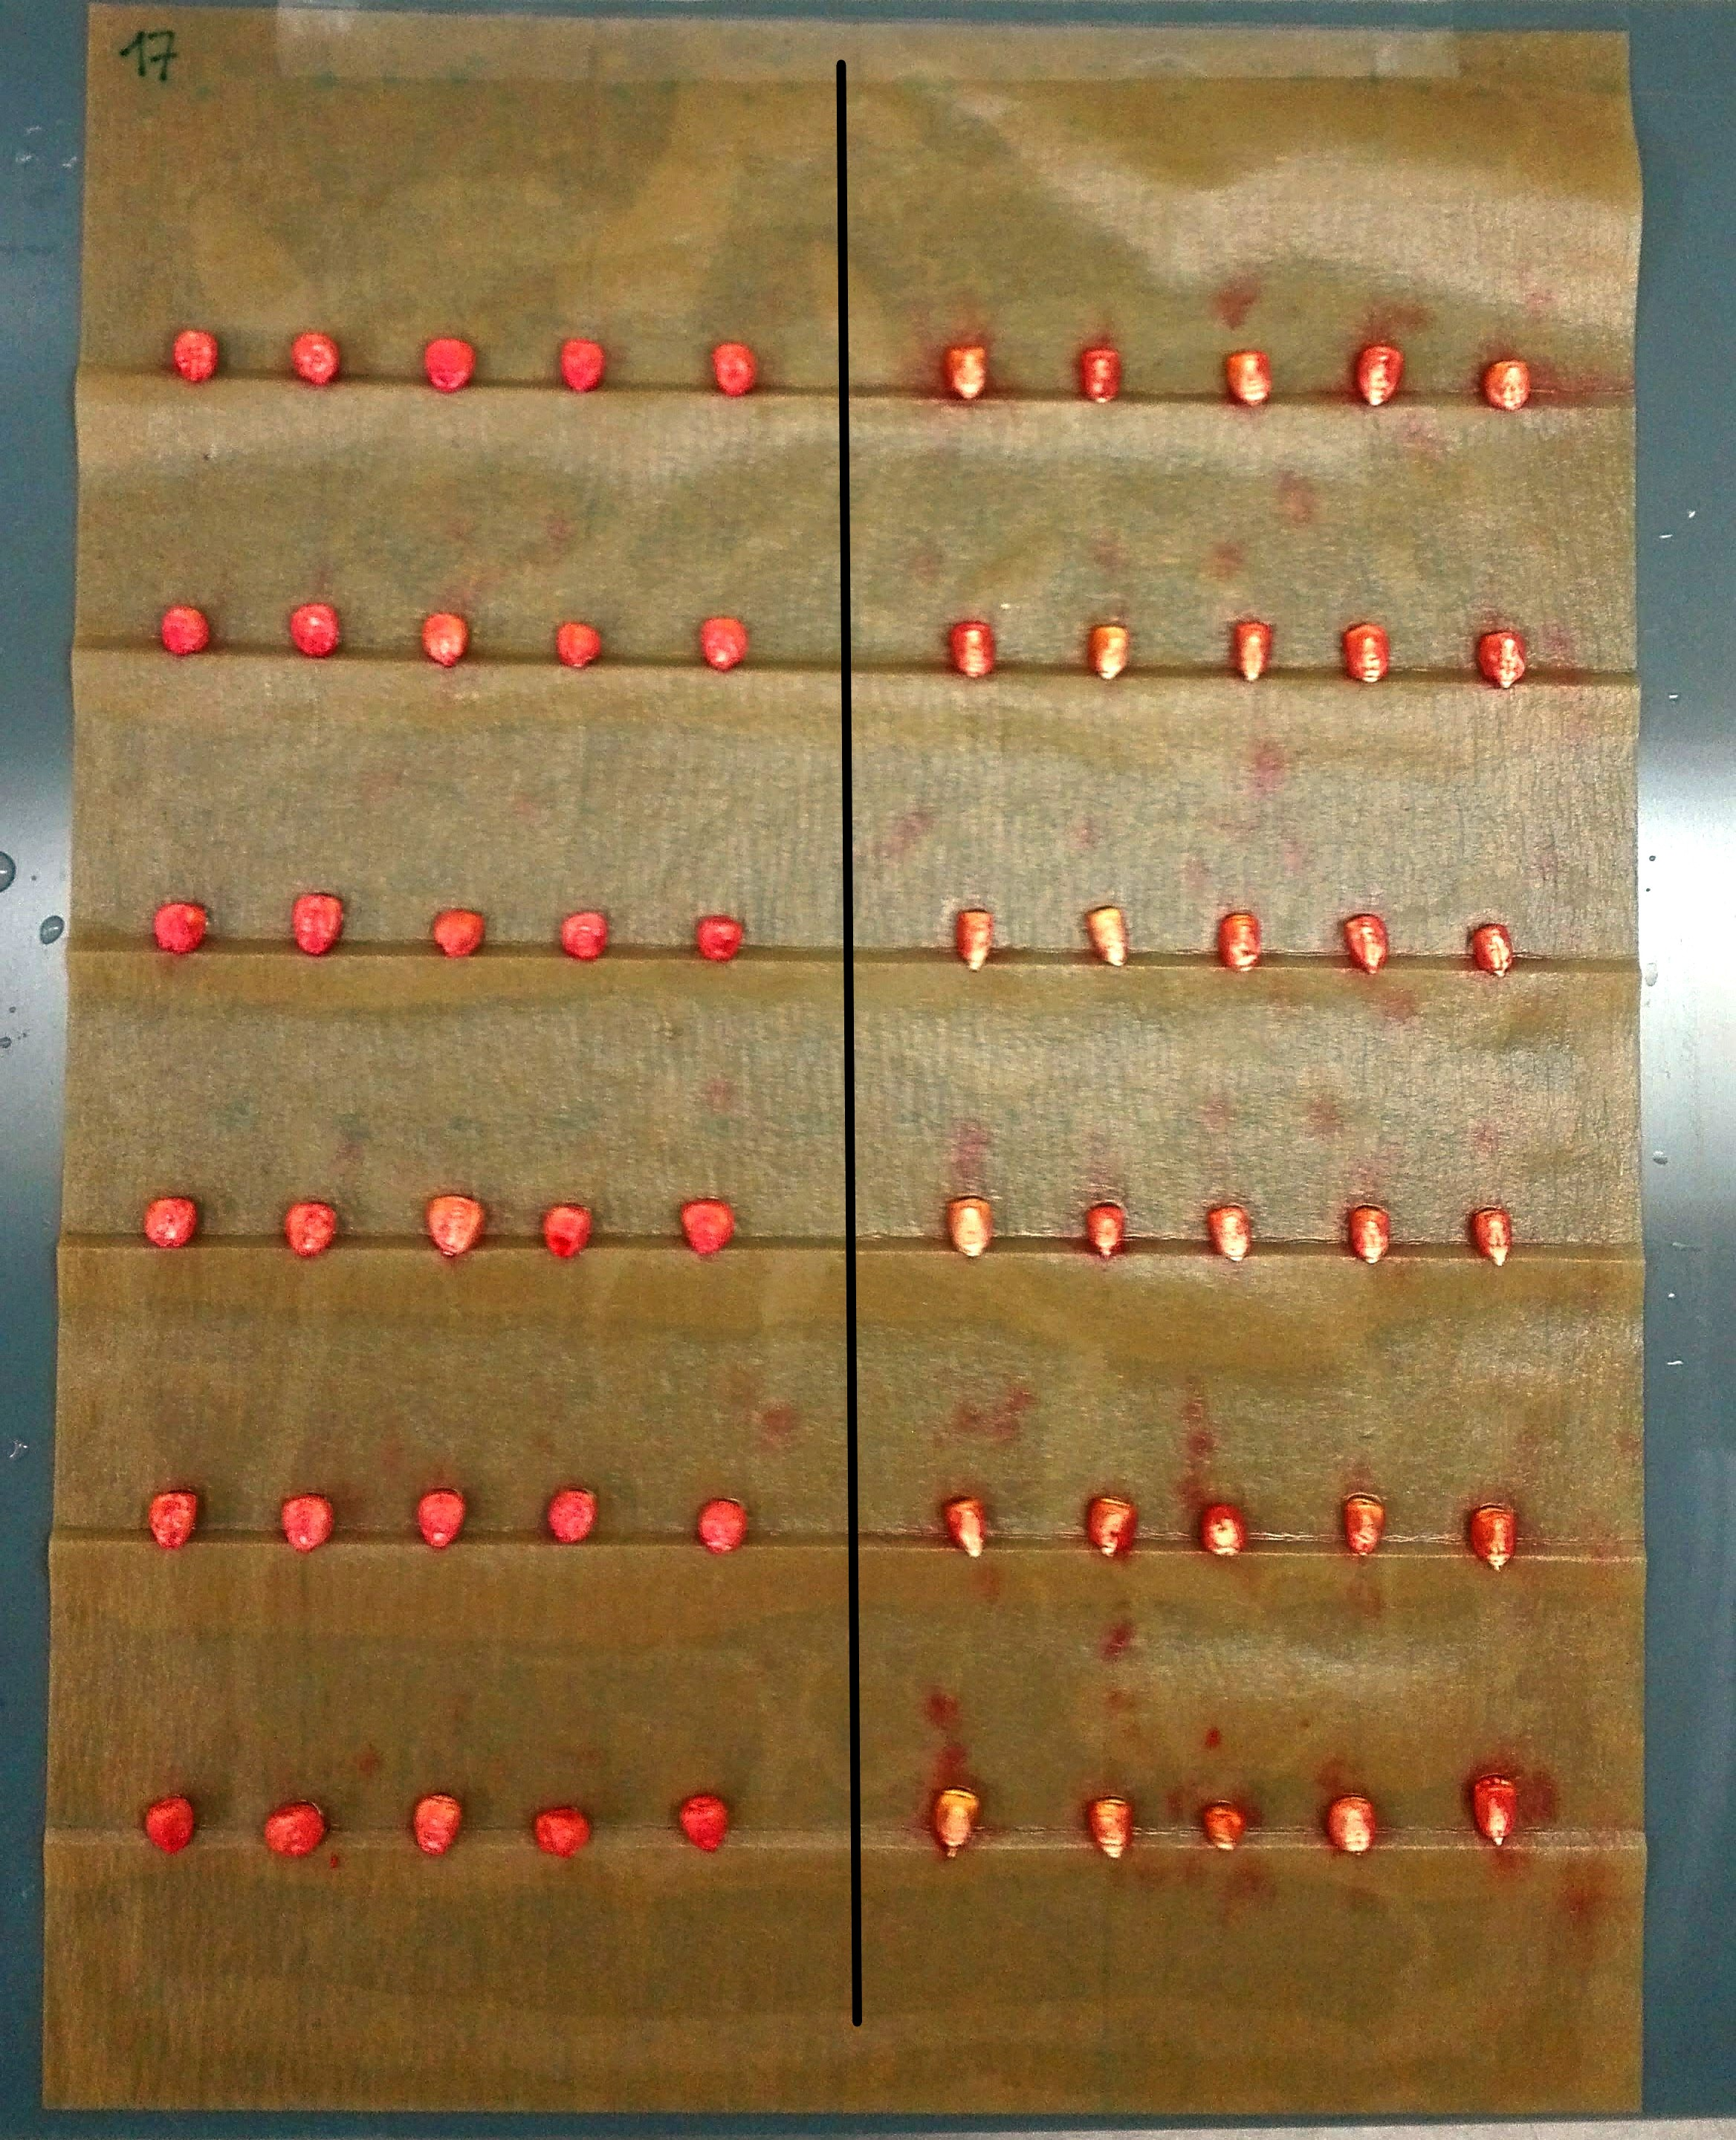
\includegraphics[width=\textwidth]{figures/photo_germination_plate.jpg}
            \caption[]%
            {30 cm by 40 cm PVC plate with seeds on filtering paper (the black line represents the separation between the two genotypes on the plate). Each sheet had 6 rows of 10 seeds with one genotype on the left and one genotype on the right.}    
            \label{fig:photo_germination_plate}
        \end{subfigure}
        \caption{Germination chamber diagram with detailed view and pictures}
    \end{figure}

After 3 days into the chamber, not all seeds were germinated, table \ref{tab:germination_percentage} presents the germination rates and mean seed weights for all the genotypes used (including the border genotype). The non-germination was mainly due to the fact that seeds fell into the water bed and because mold grew on some filtering paper.

%table for the germination rates after the outside germination process

\begin{table}[ht]
\centering
\caption{Germination rate and mean seed weight for each genotype used. (there is no data concerning the germination rate of the border genotype because it was not measured).}

\rowcolors{2}{gray!25}{white}

\begin{tabular}{lcc}
  \toprule
  %\rowcolor{gray!50}
Genotype & Germination rate (\%) & Mean seed weight (g) \\ 
  \midrule
1 & 80.00 & 0.28 \\ 
  2 & 86.67 & 0.36 \\ 
  3 & 96.67 & 0.36 \\ 
  4 & 73.33 & 0.28 \\ 
  5 & 100.00 & 0.32 \\ 
  6 & 96.67 & 0.24 \\ 
  7 & 96.67 & 0.19 \\ 
  8 & 70.00 & 0.31 \\ 
  9 & 96.67 & 0.33 \\ 
  10 & 96.67 & 0.25 \\ 
  11 & 60.00 & 0.33 \\ 
  12 & 93.33 & 0.27 \\ 
  13 & 90.00 & 0.24 \\ 
  14 & 86.67 & 0.31 \\ 
  15 & 56.67 & 0.35 \\ 
  16 & 90.00 & 0.28 \\ 
  17 & 90.00 & 0.30 \\ 
  18 & 86.67 & 0.26 \\ 
  19 & 100.00 & 0.26 \\ 
  20 & 86.67 & 0.28 \\ 
  21 & 86.67 & 0.32 \\ 
  22 & 53.33 & 0.30 \\ 
  23 & 73.33 & 0.28 \\ 
  24 & 100.00 & 0.16 \\ 
  25 & 96.67 & 0.19 \\ 
  26 & 96.67 & 0.25 \\ 
  27 & 96.67 & 0.28 \\ 
  28 & 83.33 & 0.36 \\ 
  29 & 93.33 & 0.30 \\ 
  30 & 73.33 & 0.35 \\ 
  31 & / & 0.38 \\ 
   \bottomrule
\end{tabular}
\label{tab:germination_percentage}
\end{table}

\subsection{Phenotyping platform}
The phenotyping platform is located inside a greenhouse in the facilities of the UCLouvain (Louvain-la-Neuve, Belgium). 
It consists of two aeroponic tanks on which are arranged 99 styrofoam strips, each with five holes ($\diameter$ 2.5 cm). 
At the end of each tank is a high definition camera that scans the root system of each plant individually, when it passes in front of it (fig. \ref{fig:tank}). 
The strips rotate in a clockwise fashion in the tank and a full rotation is completed in 2 hours. 
Three sprinklers are placed regularly at the bottom of each side of the tank (fig. \ref{fig:tank_transversal_view}). 
The sprinklers spray nutrient solution\footnote{The precise concentration of the Hoagland solution is presented in appendix \ref{appendix:hoagland}} at regular intervals, set by the operator. 
The spraying pattern (interval and duration) can be differentiated between day and night and can be modified at any moment of the experiment.
In this case the patterns were 5 seconds of spraying ever 295 seconds all the time.
During the experiment, the temperature of the greenhouse was set to 20$^{\circ}$C at day and 18$^{\circ}$C at night and the lights were on from 6 AM to 10 PM. 
At the start of the experiment seeds are placed inside a foam cork and then placed inside a hole on a strip (fig \ref{fig:seed_platform_close_up}). 
They are placed at the bottom to allow the root system to grow freely. 
The corks are drilled vertically to let the leaf system develop with less resistance and allow a direct access to sunlight. 
More information about the platform is available in appendix \ref{appendix:platform_info}.

After 3 days in the germination chamber, the germinated seeds were transferred onto the platform following the created design, and the non-germinated seeds were discarded. The first tank was constantly moving but only scanning the root systems once a day, while the second tank was only moving once a day to scan the root system of the plants and stayed still the rest of the day.

\begin{figure}[!htb]
        \centering
        \begin{subfigure}[b]{0.95\textwidth}
            \centering
            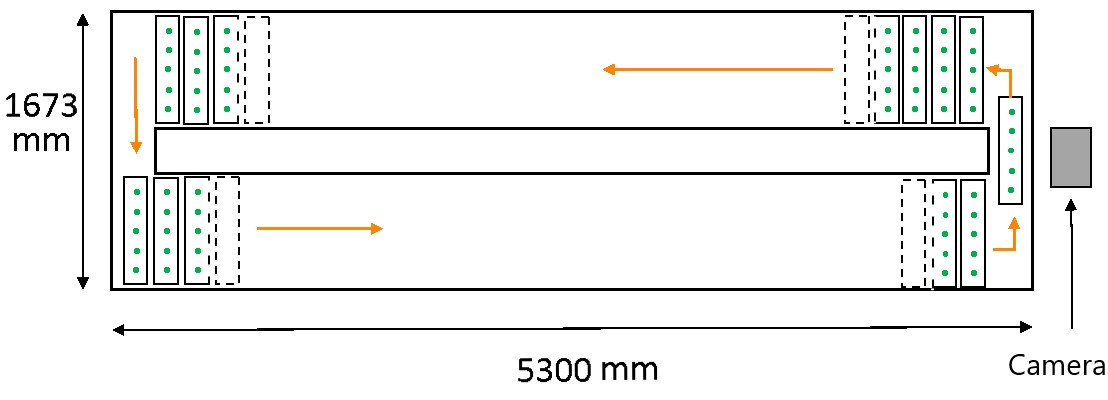
\includegraphics[width=\textwidth]{figures/tank.jpg}
            \caption{Schematic view of an aeroponic tank: plants are hold on strips, 5 plants per strip (green dots on layout). There are 99 strips in the tank for a total of 495 plants/tank. Strips move in the direction indicated by orange arrows}    
            \label{fig:tank}
        \end{subfigure}
        \vskip\baselineskip
        \begin{subfigure}[b]{0.475\textwidth}   
            \centering
            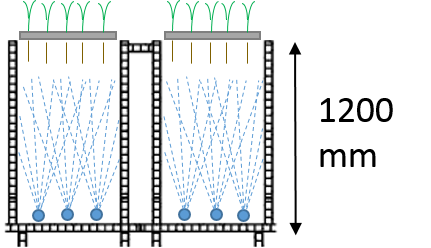
\includegraphics[width=\textwidth]{figures/tank_transversal_view.png}
            \caption{Transversal schematic view of an aeroponic tank of the platform: at the bottom of each tank, sprinklers (represented in blue in the layout) are disposed at regular interval and spray nutritive solution}    
            \label{fig:tank_transversal_view}
        \end{subfigure}
        \quad
        \begin{subfigure}[b]{0.475\textwidth}   
            \centering
            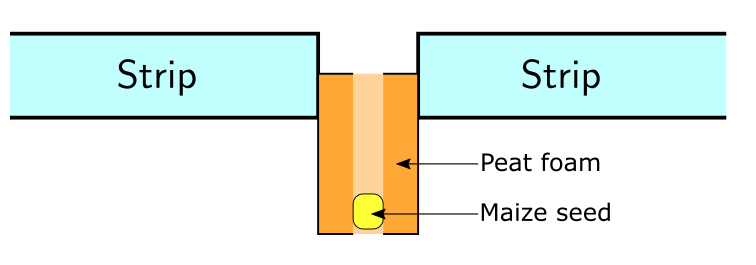
\includegraphics[width=\textwidth]{figures/seed_platform_close_up.png}
            \caption{Close up schematic view of a strip: inside each hole, seeds are placed inside a pierced peatfom cork to allow the root system to develop frelly}    
            \label{fig:seed_platform_close_up}
        \end{subfigure}
        \caption{Detailed diagrams about the phenotyping platform}
    \end{figure}


\section{Data processing}
After 15 days, the plants were considered fully grown and the experiment was stopped. The leaf and root systems were separated and weighted individually on scales precise to 0.001 g. They were then stored in individual envelopes and put in a stove at 70$^{\circ}$C for 3 days to dry. After the drying process, they were weighted again. For each plant, the remaining of the seed was consistently kept on the root system.

Two kind of data were obtained from the experiment: weight data (dry and fresh) of the fully grown plants and root scan data. Five variables were kept for the analysis:

\begin{itemize}
\item $FRESH\_RS$: fresh weight of the root system
\item $FRESH\_LS$: fresh weight of the leaf system
\item $DRY\_RS$: dry weight of the root system
\item $DRY\_LS$: dry weight of the leaf system
\item $AREA$: percentage of the total area occupied by the root system
\end{itemize} 

To be used as inputs in the models, those data need to be processed. The following sections details this step.

\subsection{Weight data}
For some plants, the germinated seeds placed on the platform did not fully grow or had an abnormal growth, but all the plants were still weighted to avoid leaving out any data. Therefore some data points need to be handled more carefully, as they do not represent the genotype's growth correctly. However, a correct growth, representative of the genotype, is hard to define because the influence of the conditions on each genotype is unknown. Therefore, instead of choosing which plants are outliers in a binary way, we attributed weights to each plant to express the quality of the data. Those weights were established by reviewing the final root scan of each plant and checking the different factors that could have an influence. The factors chosen are the following:

\begin{itemize}
\item $NO\_RS$: no additional root to the primary root
\item $NO\_LS$: no visible leaf system 
\item $BAD\_LS$: leaf system grew under the strip
\item  $NO\_SEED$: no seed (or an empty cork) present on this position
\item $NOT\_FG$: plant not fully grown
\item $OVERLAP$: leaf (or root) system of another plant overlaps on the root scan
\item $OK$: no influential factors
\end{itemize} 

An visualization of those factors with example pictures is presented in figure \ref{fig:example_influential_factors}. Some plants were attributed several influential factors, but $OK$, $NO\_SEED$ and $NOT\_FG$ were considered as exclusive. The factor attribution was ambiguous for some pictures, in those cases the plant were considered $OK$ to avoid losing any data points.
Following the determination of the factors, weights were attributed to each variable according to the weight matrix, presented in table \ref{tab:weight_attribution_matrix}.

% Table generated by Excel2LaTeX from sheet 'weights'
\begin{table}[htbp]
  \centering
  \caption{Weight attribution matrix for the different factors and variables. LS weight is both the fresh and dry weight for leaf system and RS weight is the same for the root system}
    \begin{tabular}{lrrr}
    \toprule
    CODE  & \multicolumn{1}{l}{LS weight} & \multicolumn{1}{l}{RS weight} & \multicolumn{1}{l}{Area} \\
    \midrule
    NO\_RS & 1     & 1     & 1 \\
    NO\_LS & 2     & 2     & 2 \\
    BAD\_LS & 3     & 3     & 3 \\
    NOT\_FG & 4     & 4     & 4 \\
    \textcolor[rgb]{ 1,  0,  0}{NO\_SEED} & \textcolor[rgb]{ 1,  0,  0}{0} & \textcolor[rgb]{ 1,  0,  0}{0} & \textcolor[rgb]{ 1,  0,  0}{0} \\
    \textcolor[rgb]{ 0,  .69,  .314}{OK} & \textcolor[rgb]{ 0,  .69,  .314}{5} & \textcolor[rgb]{ 0,  .69,  .314}{5} & \textcolor[rgb]{ 0,  .69,  .314}{5} \\
    OVERLAP & 1     & 1     & 0 \\
    \bottomrule
    \end{tabular}%
  \label{tab:weight_attribution_matrix}%
\end{table}%


\begin{sidewaysfigure}[ht]
\centering
\begin{subfigure}[t]{.13\textwidth}
  \centering
  \includegraphics[width=\linewidth]{figures/NO_RS.jpg}
  \caption{$NO_RS$: no additional root, other than the primary}
  \label{fig:NO_RS}
\end{subfigure}
%
\begin{subfigure}[t]{.13\textwidth}
  \centering
  \includegraphics[width=\linewidth]{figures/NO_LS.jpg}
  \caption{$NO\_LS$: no apparent leaf system}
  \label{fig:NO_LS}
\end{subfigure}
%
\begin{subfigure}[t]{.13\textwidth}
  \centering
  \includegraphics[width=\linewidth]{figures/BAD_LS.jpg}
  \caption{$BAD\_LS$: the leaf system grew under the strip and deviated to the right (obstruction of another plant)}
  \label{fig:BAD_LS}
\end{subfigure}
%
\begin{subfigure}[t]{.13\textwidth}
  \centering
  \includegraphics[width=\linewidth]{figures/NO_SEED.jpg}
  \caption{$NO\_SEED$}
  \label{fig:NO_SEED}
\end{subfigure}
%
\begin{subfigure}[t]{.13\textwidth}
  \centering
  \includegraphics[width=\linewidth]{figures/NOT_FG.jpg}
  \caption{$NOT\_FG$: both system are present but underdeveloped compared to other images }
  \label{fig:NOT_FG}
\end{subfigure}
%
\begin{subfigure}[t]{.13\textwidth}
  \centering
  \includegraphics[width=\linewidth]{figures/OVERLAP.jpg}
  \caption{$OVERLAP$: the leaf system of another plant hides the root system of the plant}
  \label{fig:OVERLAP}
\end{subfigure}
%
\begin{subfigure}[t]{.13\textwidth}
  \centering
  \includegraphics[width=\linewidth]{figures/OK.jpg}
  \caption{$OK$, the green box represents the bounding area for the computation of the root area}
  \label{fig:OK}
\end{subfigure}
%
\caption{Example pictures of the influential factors chosen for the weight attribution.}
\label{fig:example_influential_factors}
\end{sidewaysfigure}

\subsection{Root pictures}
The area of the root system was computed using the final root scan of each plant. Each picture was converted to gray-scale, resized to a specific bounding rectangle and binarized. The bounding box is illustrated on figure \ref{fig:OK}. The threshold for the binarization was 140 on a 0 to 255 scale. Since the roots are black on the original picture, the binarization was completed without any issues. The area of the root system was expressed as a percentage of the total area of the bounding box, by counting the black pixels in the image. All the processing was done in python using the opencv package.


\section{SpATS model}
In this section, the SpATS model is introduced. For a more thorough treatment of the model and all its components, see \textcite{rodriguez2016spatial}.\\
Consider a field trial of $n$ plots arranged in a rectangular grid, where the plot positions are collected in vectors of row $(\mathbf{r})$ and column $(\mathbf{c})$ coordinates. If $\mathbf{y}$ is the vector of plot data in field order, a common model for $\mathbf{y}$, to use as a starting point is
\begin{equation}
    \boldsymbol{y}=\mathbf{1}_{n} \beta_{0}+\boldsymbol{Z}_{r} \boldsymbol{c}_{r}+\boldsymbol{Z}_{c} \boldsymbol{c}_{c}+\varepsilon
\end{equation}
were $\mathbf{1}_{n}$ is a column-vector of ones of length $n$, $\boldsymbol{c}_{r}$ and $\boldsymbol{c}_{c}$ are, respectively, the random effect coefficients for the rows and columns and associated matrix $\boldsymbol{Z}_{r}$ and $\boldsymbol{Z}_{c}$. To fully capture complex spatial patterns, a smooth bivariate surface jointly defined over the row and column positions is added to the model, which becomes
\begin{equation}
    \boldsymbol{y}=f(\boldsymbol{u}, \boldsymbol{v})+\boldsymbol{Z}_{r} \boldsymbol{c}_{r}+\boldsymbol{Z}_{c} \boldsymbol{c}_{c}+\boldsymbol{\varepsilon}
    \label{eq:base_model_bismooth_surface}
\end{equation}
where $\mathbf{u}$ and $\mathbf{v}$ are, respectively, the vector of row and columns positions and where $f(.,.)$ represents the smooth bivariate function. Note that the intercept term, $\beta_0$ is embedded into $f(u,v)$. To better understand this function, let us decompose it in a nested-ANOVA structure
\begin{align}
f ( \boldsymbol { u } , \boldsymbol { v } ) & = \underbrace { \mathbf { 1 } _ { n } \beta _ { 0 } + \boldsymbol { u } \beta _ { 1 } + \boldsymbol { v } \beta _ { 2 } + \boldsymbol { u } \odot \boldsymbol { v } \beta _ { 3 } } _ { \text { Bilinear polynomial } } \nonumber \\
 & + \underbrace { f _ { u } ( \boldsymbol { u } ) + f _ { v } ( \boldsymbol { v } ) + \boldsymbol { u } \odot h _ { v } ( \boldsymbol { v } ) + \boldsymbol { v } \odot h _ { u } ( \boldsymbol { u } ) + f _ { u , v } ( \boldsymbol { u } , \boldsymbol { v } ) }_{\text{Smooth part}}
 \label{eq:full_bivariate_smooth_surface_model}
\end{align}
where $\odot$ denotes the element-wise matrix product\footnote{See Appendix A for details about the element-wise matrix product.}. There are now two components to the model: a bilinear polynomial part(parametric) and a smooth part (non-parametric). The parametric part includes the linear trends along rows ($\beta_1$) and columns ($\beta_2$) as well as a linear interaction trend ($\beta_3$). The smooth part models the deviation from the compound linear trend, and can be decomposed in the following elements:
\begin{itemize}
\item $f _ { u } ( \boldsymbol { u } )$  is a smooth trend along the rows, identical for all columns (i.e., a main smooth effect).
\item $f _ {v} ( \boldsymbol { v} )$ is a smooth trend along the columns, identical for all rows.
\item $\boldsymbol { v } \odot h _ { u } ( \boldsymbol { u } ))$ and $\boldsymbol { u } \odot h _ { v } ( \boldsymbol { v } )$ are linear-by-smooth interaction trends. For instance, $\boldsymbol { u }h_\boldsymbol { v}(\boldsymbol { v})$ is a varying coefficient surface trend, consisting of functions, linear in the rows, for each column, but with slopes that change smoothly along the columns, $h_\boldsymbol { v}(\boldsymbol { v})$.
\item $f _ { u , v } ( \boldsymbol { u } , \boldsymbol { v } )$ is a smooth-by-smooth interaction trend jointly defined over the row and column directions.
\end{itemize}
In total, six components are used to model the surface $f$. This may seem like a lot but this allows the translation of model \ref{eq:base_model_bismooth_surface} into a standard mixed model. An interesting property of this proposal is that since $u$ and $v$ are row and column position, it allows depicting the spatial trend in a grid finer than the number of rows and columns.

\subsection{Modelling using P-splines}
The functions $f_u$, $f_v$, $h_u$ and $h_v$ are constructed  with variations on one-dimensional P-splines, while $f_{u,v}$ is based on tensor products P-splines.\\
For clarity's sake, let us consider a model only containing a smooth bivariate surface and an error term
\begin{equation}
    y _ { i } = f \left( u _ { i } , v _ { i } \right) + \varepsilon _ { i } , \text { with } \varepsilon _ { i } \sim N \left( 0 , \sigma ^ { 2 } \right) \text{.}
\label{eq:smooth_part_only_model}
\end{equation}
\textcite{lee_efficient_2013} show that it can be represented using B-splines\footnote{See Appendix A for details about B-splines and P-splines.}. Let us form two B-splines basis:
\begin{enumerate}
\item one for the columns, $\boldsymbol{\invbreve{B}}$ with $ b_{il}= \invbreve{B}_l(u_i)$, where $\invbreve{B}_l(u_i)$ is the $l$th B-spline of the basis, evaluated at $u_i$
\item and one for the rows, $\boldsymbol{\breve{B}}$ with $ b_{ip}= \breve{B}_p(v_i)$, where $\breve{B}_l(v_i)$ is the $p$th B-spline of the basis, evaluated at $v_i$.
\end{enumerate}
Then, the smooth-by-smooth interaction can be written using those basis
\begin{equation}
f \left( u _ { i } , v _ { i } \right) = \sum _ { l = 1 } ^ { L } \sum _ { p = 1 } ^ { P } \invbreve { B } _ { l } \left( u _ { i } \right) \breve { B } _ { p } \left( v _ { i } \right) \alpha _ { l p }  \text{,}
\end{equation}
where $\boldsymbol{\alpha} = (\alpha_{11},\ldots,\alpha_{1P},\ldots,\alpha_{LP})^t$ is a vector of unknown regression coefficients of dimension $(LP \times 1)$. Note that $\boldsymbol{\invbreve{B}}$ and $\boldsymbol{\breve{B}}$ are matrices of order $n \times L$ and $n\times P$ respectively, where $L$ and $P$ are the number of the B-spline basis functions. \textcite{dierckx_curve_1995} shows that, in the P-spline framework, the smooth-by-smooth interaction $f(u_i,v_i)$ is modelled by the tensor product of B-splines bases. Then, we can write, in matrix notation,
\begin{equation}
    \boldsymbol{B} = \boldsymbol{\invbreve{B}} \square \boldsymbol{\breve{B}} = \left( \boldsymbol{\invbreve{ B }} \otimes \boldsymbol{1} _ { L } ^ { t } \right) \odot \left( \mathbf { 1 } _ { P } ^ { t } \otimes \boldsymbol{\breve{B}} \right) \text{,}
\end{equation}
where the operation $\square$ is defined in terms of the Kronecker product of two matrices (denoted by $\otimes$) and the element-by-element multiplication of two matrices (denoted by $\odot$)\footnote{See Appendix A for details about the Kronecker product}. Therefore model (\ref{eq:smooth_part_only_model}) can be written in matrix notation
\begin{equation}
    \boldsymbol{y} = \boldsymbol{B}\boldsymbol{\alpha} + \boldsymbol{\epsilon}
    \text{.}
    \label{eq:spline_model_mat_form}
\end{equation}
Since the model is purely parametric, it can be estimated by minimizing the residual sum of squares (with explicit solution $\Hat{\boldsymbol{\alpha}} = (\mathbf{B}^t\mathbf{B})^{-1}\mathbf{B}^t\mathbf{y}$). To prevent over-fitting, \textcite{eilers_flexible_1996} propose to incorporate a discrete penalty on the coefficient associated to adjacent B-splines. For the two-dimensional case, the vector $\boldsymbol{\alpha}$ can be seen as an  $(L \times P)$  matrix  of  coefficients, $\mathbf{A}=[\alpha_{lp}]$. Now the rows  and columns of $\mathbf{A}$ correspond to the regression coefficients in the $v$ and  $u$ direction, respectively. In anisotropic (direction-dependant) P-splines, a different amount of smoothing is assumed along the $u$ and $v$ directions. It leads to two penalties:  one on all rows of $\mathbf{A}$,  the other on all of its columns; and the penalized least squares objective function becomes \parencite{eilers_multivariate_2003}
\begin{equation}
    S^{*}=\|\boldsymbol{y}-\boldsymbol{B} \boldsymbol{\alpha}\|^{2}+\invbreve{\lambda}\|\invbreve{\boldsymbol{D}} A\|_{F}^{2}+\breve{\lambda}\left\|\boldsymbol{A} \breve{D}^{t}\right\|_{F}^{2}=\|\boldsymbol{y}-\boldsymbol{B} \boldsymbol{\alpha}\|^{2}+\boldsymbol{\alpha}^{t} \boldsymbol{P} \boldsymbol{\alpha}
    \text{,}
    \label{eq:least_squares_penalized}
\end{equation}
where $\boldsymbol{P}=\invbreve{\lambda}\left(\boldsymbol{I}_{P} \otimes \invbreve{\boldsymbol{D}}^{t} \invbreve{\boldsymbol{D}}\right)+\breve{\lambda}\left(\breve{\boldsymbol{D}}^{t} \breve{\boldsymbol{D}} \otimes \boldsymbol{I}_{L}\right)$ is the penalty matrix, $\invbreve{\lambda}$ and $\breve{\lambda}$ are the smoothing parameters acting, respectively, on the columns and rows of $\mathbf{A}$, and $\invbreve{\mathbf{D}}$ and $\breve{\mathbf{D}}$ are the matrices that form differences of order $d_u$ and $d_v$ respectively\footnote{See appendix A for more information about penalized splines and ordered differences}. The minimizer of \ref{eq:least_squares_penalized} is 
\begin{equation}
    \widehat{\boldsymbol{\alpha}}=\left(\boldsymbol{B}^{t} \boldsymbol{B}+\boldsymbol{P}\right)^{-1} \boldsymbol{B}^{t} \boldsymbol{y}
    \text{.}
\end{equation}
The advantage of this decomposition is that the only tuning parameters for the smoothness of the bivariate surface are the smoothing parameters $\invbreve{\lambda}$ and $\breve{\lambda}$.

\subsection{Mixed model based smoothing parameter selection}

As explained in \textcite{rodriguez2016spatial}, $\mathbf{P}$ is rank-deficient and this causes numerical instability when applying mixed model estimation techniques. To obtain a full-rank penalty matrix, the key is to write model \ref{eq:spline_model_mat_form} as 
\begin{equation}
    \mathbf{B}\boldsymbol{\alpha} = \boldsymbol{X}_{s} \boldsymbol{\beta}_{s}+\boldsymbol{Z}_{s} \boldsymbol{c}_{s}
    \text{.}
\end{equation}
There are now two bases: $\mathbf{X}_{s}$, with coefficients that are not penalized at all, and $\mathbf{Z}_{s}$, with a size penalty on its coefficients. This decomposition follows the proposal by \textcite{lee_p-spline_2011}, based on eigenvalue decomposition which gives rise to a diagonal penalty matrix.\\
Let $\invbreve{D}^{t} \invbreve{D}=U_{u} E_{u} U_{u}^{t}$ and $\breve{D}^{t} \breve{D}=U_{v} E_{v} U_{v}^{t}$ be the eigenvalue decomposition of the marginal penalties, $\invbreve{D}^{t} \invbreve{D}$ and $\breve{D}^{t} \breve{D}$, respectively. Here $\mathbf{U}_{j}$ denotes the matrix of eigenvectors and $\mathbf{E}_j$  the diagonal matrix of eigenvalues $(j=u,v)$. Let us denote $\widetilde{\boldsymbol{U}}_{j}$ and $\widetilde{\boldsymbol{E}}_{j}$ the sub-matrices corresponding to non-zero eigenvalues. Setting
\begin{equation}
    \boldsymbol{X}_{s}=\left[\mathbf{1}_{n}, \boldsymbol{u}, \boldsymbol{v}, \boldsymbol{u} \odot \boldsymbol{v}\right]
    \quad
    \text{and}
    \quad
    \mathbf{Z}_{s}=\left[\mathbf{Z}_{v}, \mathbf{Z}_{u}, \mathbf{Z}_{v} \square \mathbf{u}, \mathbf{v} \square \mathbf{Z}_{u}, \mathbf{Z}_{v} \square \mathbf{Z}_{u}\right]
    \text{,}
    \label{eq:detail_Xs_Zs_matrices}
\end{equation}
where $\mathbf{Z}_u = \breve{\mathbf{B}}\widetilde{\boldsymbol{U}}_{u}$ and $\mathbf{Z}_v = \breve{\mathbf{B}}\widetilde{\boldsymbol{U}}_{v}$, the penalized least problem (\ref{eq:least_squares_penalized}) becomes
\begin{equation}
    S^{*}=\left\|\boldsymbol{y}-\boldsymbol{X}_{s} \boldsymbol{\beta}_{s}-\boldsymbol{Z}_{s} \boldsymbol{c}_{s}\right\|^{2}+\boldsymbol{c}_{s}^{t} \widetilde{\boldsymbol{P}} \boldsymbol{c}_{s}
    \text{,}
    \label{eq:new_least_squares_penalized}
\end{equation}
where
\begin{equation}
    \widetilde{\boldsymbol{P}} = \text{blockdiag}\left(\breve{\lambda} \widetilde{\boldsymbol{E}}_{v}, \invbreve{\lambda} \widetilde{\boldsymbol{E}}_{u}, \breve{\lambda} \widetilde{\boldsymbol{E}}_{v}, \invbreve{\lambda} \widetilde{\boldsymbol{E}}_{u}, \breve{\lambda} \widetilde{\boldsymbol{E}}_{v} \otimes \boldsymbol{I}_{L-2}+\invbreve{\lambda} \boldsymbol{I}_{P-2} \otimes \widetilde{\boldsymbol{E}}_{u}\right)
    \text{,}
\end{equation}
is the new penalty matrix. Each block of $\widetilde{\boldsymbol{P}}$ corresponds to a block in $\mathbf{Z}_s$. This reformulation provides the ANOVA type decomposition discussed in the previous section (\ref{eq:full_bivariate_smooth_surface_model}). The block structure of $\mathbf{X}_s$ and $\mathbf{Z}_s$ implies
\begin{equation}
    \begin{aligned} 
        f(\boldsymbol{u}, \boldsymbol{v}) &
        =\boldsymbol{X}_{s} \boldsymbol{\beta}_{s}+Z_{s} \boldsymbol{c}_{s} \\ 
        &=\mathbf{1}_{n} \beta_{0}+\boldsymbol{u} \beta_{1}+\boldsymbol{v} \beta_{2}+\boldsymbol{u} \odot \boldsymbol{v} \beta_{3} \\
        & + \underbrace{f_{v}(\boldsymbol{v})}_{\boldsymbol{Z}_{v} \boldsymbol{c}_{s 1}}+\underbrace{f_{u}(\boldsymbol{u})}_{\boldsymbol{Z}_{u} \boldsymbol{c}_{s 2}} +\underbrace{\boldsymbol{u} \odot h_{v}(\boldsymbol{v})}_{\left[\boldsymbol{Z}_{v} \square \boldsymbol{u}\right] \boldsymbol{c}_{s 3}}+\underbrace{\boldsymbol{v} \odot h_{u}(\boldsymbol{u})}_{\left[\boldsymbol{v} \square \boldsymbol{Z}_{u}\right] \boldsymbol{c}_{s 4}} +\underbrace{f_{u, v}(\boldsymbol{u}, \boldsymbol{v})}_{\left[\boldsymbol{Z}_{v} \square \boldsymbol{Z}_{u}\right] \boldsymbol{c}_{s 5}}
        \text{,}
    \end{aligned}
\end{equation}
where $\boldsymbol{c}_{sk} \ (k = 1,\ldots,5)$ contains the elements of $\boldsymbol{c}_s$ that correspond to the $k$th block of $\boldsymbol{Z}_s$, i.e. $\boldsymbol{c}_s = (\boldsymbol{c}_{s1}^t,\ldots,\boldsymbol{c}_{s5}^t)^t$.\\
The solution for \ref{eq:new_least_squares_penalized}, given $\breve{\lambda}$ and $\invbreve{\lambda}$, corresponds to the best linear unbiased estimator (BLUE) for the $(4\times1)$ vector $\boldsymbol{\beta}_s$, and the BLUPs for the $((LP - 4) \times 1)$ vector $\boldsymbol{c}_s$ under the linear mixed model
\begin{equation}
    \boldsymbol{y}=\boldsymbol{X}_{s} \boldsymbol{\beta}_{s}+\boldsymbol{Z}_{s} \boldsymbol{c}_{s}+\boldsymbol{\varepsilon}, \text { with } \boldsymbol{\varepsilon} \sim N\left(\mathbf{0}, \sigma^{2} \boldsymbol{I}_{n}\right) \text { and } \boldsymbol{c}_{s} \sim N\left(\mathbf{0}, \boldsymbol{G}_{s}\right)
    \text{,}
\end{equation}
where $\boldsymbol{G}_{s} = \sigma^2\widetilde{\boldsymbol{P}}^{-1}$. Denoting $\breve{\sigma}^2 =\sigma / \breve{\lambda}$ and $\invbreve{\sigma}^2 =\sigma / \invbreve{\lambda}$ the variances parameters involved in $\boldsymbol{G}_{s}$, it follows
\begin{equation}
    \boldsymbol{G}_s^{-1} = \text{blockdiag}\left(\frac{1}{\breve{\sigma}^{2}} \widetilde{\boldsymbol{E}}_{v}, \frac{1}{\invbreve{\sigma}^{2}} \widetilde{\boldsymbol{E}}_{u}, \frac{1}{\breve{\sigma}^{2}} \widetilde{\boldsymbol{E}}_{v}, \frac{1}{\invbreve{\sigma}^{2}} \widetilde{\boldsymbol{E}}_{u}, \frac{1}{\breve{\sigma}^{2}} \widetilde{\boldsymbol{E}}_{v} \otimes \boldsymbol{I}_{L-2}+\frac{1}{\invbreve{\sigma}^{2}} \boldsymbol{I}_{P-2} \otimes \widetilde{\boldsymbol{E}}_{u}\right)
    \text{.}
\end{equation}
Note that besides the five smooth components, $\mathbf{G}_s$ involves only two variance parameters, $\breve{\sigma}^2$ and $\invbreve{\sigma}^2$. In fact, the same variance parameters control the smoothness of the both the main effects and interactions terms. This prevents the use of standard mixed models software for estimation since $\mathbf{G}_s$ has its last block depending on both $\breve{\sigma}^2$ and $\invbreve{\sigma}^2$, but in a non-linear way. Even though \textcite{rodriguez2015fast} presented a specialized algorithm to deal with this issue, here the PS-ANOVA decomposition approach \parencite{lee_efficient_2013} is used to allow the use of standard mixed model estimation procedures. \textcite{lee_efficient_2013} therefore propose to use a different variance component for each smooth component in $\mathbf{G}_s$. Denoting 
$\mathbf{\Lambda}_{s 1}^{-1}=\mathbf{\Lambda}_{s 3}^{-1}=\widetilde{E}_{v}, \mathbf{\Lambda}_{s 2}^{-1}=\mathbf{\Lambda}_{s 4}^{-1}=\widetilde{\boldsymbol{E}}_{u}, \text { and } \mathbf{\Lambda}_{s 5}^{-1}=\widetilde{\boldsymbol{E}}_{v} \otimes \boldsymbol{I}_{L-2}+\boldsymbol{I}_{P-2} \otimes \widetilde{\boldsymbol{E}}_{u}$
the precision matrix, $\boldsymbol{G}_s^{-1}$, is then redefined as
\begin{equation}
    \mathbf{G}_{s}^{-1}=\text { blockdiag }\left(\frac{1}{\sigma_{s 1}^{2}} \mathbf{\Lambda}_{s 1}^{-1}, \frac{1}{\sigma_{s 2}^{2}} \mathbf{\Lambda}_{s 2}^{-1}, \frac{1}{\sigma_{s 3}^{2}} \mathbf{\Lambda}_{s 3}^{-1}, \frac{1}{\sigma_{s 4}^{2}} \mathbf{\Lambda}_{s 4}^{-1}, \frac{1}{\sigma_{s 5}^{2}} \mathbf{\Lambda}_{s 5}^{-1}\right)
    \text{,}
\end{equation}
and thus the covariance matrix $\mathbf{G}_s$ is a linear function of variance parameters
\begin{equation}
    \boldsymbol{G}_{s}=\bigoplus_{k=1}^{5} \sigma_{s k}^{2} \Lambda_{s k}=\bigoplus_{k=1}^{5} \boldsymbol{G}_{s k}=
    \text{ blockdiag }
    \left(\boldsymbol{G}_{s 1}, \boldsymbol{G}_{s 2}, \boldsymbol{G}_{s 3}, \boldsymbol{G}_{s 4}, \boldsymbol{G}_{s 5}\right)
    \text{,}
\end{equation}
where $\boldsymbol{G}_{s k} = \sigma_{sk}^2\boldsymbol{\Lambda}_{sk} \ (k=1,\ldots,5)$. In other words, here the tensor product P-splines mixed model is represented as the sum of 5 sets of mutually independent Gaussian random components $\mathbf{c}_{sk}$, each depending on one variance $\sigma_{sk}^2 \ (k=1,\ldots,5)$.

\subsection{Spatial models for field trials}
The tensor product P-spline, presented in the previous section, constitutes the base for the analysis of agricultural field trials because it allows the modeling of the random spatial variation typically presented in a field. On top of this spatial field, we need to build up more complex models in order to account for the genetic variation, the presence of blocks effects, or other sources of variation (see section \ref{sec:sources_of_variation}). From now on, we therefore consider the following linear mixed model
\begin{equation}
    \boldsymbol{y}=\underbrace{\boldsymbol{X}_{s} \boldsymbol{\beta}_{s}+Z_{s} \boldsymbol{c}_{s}}_{f(\boldsymbol{u}, \boldsymbol{v})}+\boldsymbol{X}_{d} \boldsymbol{\beta}_{d}+\boldsymbol{Z}_{d} \boldsymbol{c}_{d}+\varepsilon, \text { with } \boldsymbol{c}_{s} \sim N\left(\mathbf{0}, \boldsymbol{G}_{s}\right) \text { and } \boldsymbol{c}_{d} \sim N\left(\mathbf{0}, \boldsymbol{G}_{d}\right)
    \text{,}
    \label{eq:full_random_and_additonal_effects_model}
\end{equation}
where $\boldsymbol{X}_{s}$, $\boldsymbol{Z}_{s}$ and $\boldsymbol{G}_{s}$ are defined in the previous section and where $\boldsymbol{X}_{d}$ and $\boldsymbol{Z}_{d}$ represent column-partitioned matrices, associated respectively with extra fixed and random components, as for instance, row, column, genotypic effects. We assume that $\boldsymbol{X}_{d}$ has full rank, $\boldsymbol{Z}_{d}=\left[\boldsymbol{Z}_{d 1}, \ldots, \boldsymbol{Z}_{d b}\right]$ and $\boldsymbol{c}_d = \left( \boldsymbol{c}_{d1}^t,\ldots,\boldsymbol{c}_{db}^t\right)^t$. Each $\boldsymbol{Z}_{dk}$ corresponds to the design matrix of the $k$th random component $\boldsymbol{c}_{dk}$, with $\boldsymbol{c}_{dk}$ being a $(m_{dk} \times 1)$ vector $(k=1,\ldots,b)$. We assume further that $\boldsymbol{c}_s$ and $\boldsymbol{c}_d$ are independant, and that $\boldsymbol{G}_{d}=\bigoplus_{k=1}^{b} \boldsymbol{G}_{d k}=\bigoplus_{k=1}^{b} \sigma_{d k}^{2} \mathbf{\Lambda}_{d k}$, where $\boldsymbol{\Lambda}_{dk}$ are diagonal matrices. To keep the notation simple, we rewrite model (\ref{eq:full_random_and_additonal_effects_model}) as
\begin{equation}
    \boldsymbol{y}=\boldsymbol{X} \boldsymbol{\beta}+\boldsymbol{Z} \boldsymbol{c}+\boldsymbol{\varepsilon}, \text { with } \boldsymbol{c} \sim N(\mathbf{0}, \boldsymbol{G}) \text { and } \boldsymbol{\varepsilon} \sim N\left(\mathbf{0}, \sigma^{2} \boldsymbol{I}_{n}\right)
\end{equation}
where $\boldsymbol{X}=\left[\boldsymbol{X}_{s}, \boldsymbol{X}_{d}\right], \boldsymbol{Z}=\left[\boldsymbol{Z}_{s}, \boldsymbol{Z}_{d}\right]=\left[\boldsymbol{Z}_{1}, \ldots, \boldsymbol{Z}_{q}\right] \ (q=5+b)$, and 
\begin{equation}
    \boldsymbol{G}=\text { blockdiag }\left(\boldsymbol{G}_{s}, \boldsymbol{G}_{d}\right)=\bigoplus_{k=1}^{q} \boldsymbol{G}_{k}=\bigoplus_{k=1}^{q} \sigma_{k}^{2} \boldsymbol{\Lambda}_{k}
\end{equation}

\subsection{Model estimation}
Estimates of the fixed and random effects coefficients in model \ref{eq:final_MM_eq}, for given values of the variance components, follow from standard mixed-mode theory and can be obtained by maximizing the REML log-likelihood function
\begin{equation}
    l=-\frac{1}{2} \log |\boldsymbol{V}|-\frac{1}{2} \log \left|\boldsymbol{X}^{t} \boldsymbol{V}^{-\mathbf{1}} \boldsymbol{X}\right|-\frac{1}{2}(\boldsymbol{y}-\boldsymbol{X} \widehat{\boldsymbol{\beta}})^{t} \boldsymbol{V}^{-1}(\boldsymbol{y}-\boldsymbol{X} \widehat{\boldsymbol{\beta}})
    \text{.}
\end{equation}
The implementation of this procedure in the SpATS packages is detailed in the appendix of \textcite{rodriguez2016spatial}. The REML estimates are obtained taking the derivatives of the previous equation, with respect to the variance components $\sigma_k^2 \ (k=1,\ldots,q)$ and equating the obtained expression to zero (see e.g. \cite{rodriguez2015fast,johnson1995restricted}), we obtain that
\begin{equation}
    \widehat{\sigma}_{k}^{2}=\frac{\widehat{\mathbf{c}}_{k}^{t} \boldsymbol{\Lambda}_{k}^{-1} \widehat{\mathbf{c}}_{k}}{\mathrm{ED}_{k}}, k=1, \ldots, q
\end{equation}
with
\begin{equation}
    \mathrm{ED}_{k}=\operatorname{trace}\left(\mathbf{Z}_{k}^{t} \mathbf{Q} \mathbf{Z}_{k} \mathbf{G}_{k}\right)
\end{equation}
where $\mathbf{Q}=\boldsymbol{V}^{-1}-\boldsymbol{V}^{-1} \boldsymbol{X}\left(\boldsymbol{X}^{t} \boldsymbol{V}^{-1} \boldsymbol{X}\right)^{-1} \boldsymbol{X}^{t} \boldsymbol{V}^{-1}$ with $\boldsymbol{V}=\boldsymbol{R}+\mathbf{Z}\boldsymbol{G} \mathbf{Z}^{t}$ and $\boldsymbol{R}=\sigma^{2} \boldsymbol{I}_{n}$. An estimate of $\sigma^2$ can also be easily obtained following the same reasoning
\begin{equation}
    \widehat{\sigma}^{2}=\frac{\widehat{\boldsymbol{\varepsilon}}^{t} \hat{\boldsymbol{\varepsilon}}}{\mathrm{ED}_{\boldsymbol{\varepsilon}}}
    \label{eq:var_estimation_SPATS}
\end{equation}
where $\widehat{\boldsymbol{\varepsilon}}=\mathbf{y}-\mathbf{X} \widehat{\boldsymbol{\beta}}+\mathbf{Z} \widehat{\mathbf{c}}$ and
\begin{equation}
    \mathrm{ED}_{\boldsymbol{\varepsilon}}=\operatorname{trace}(\mathbf{R Q})=n-\operatorname{rank}(\mathbf{X})-\sum_{k=1}^{q} \mathrm{ED}_{k}
    \text{.}
    \label{eq:ED_error_term}
\end{equation}
In these equations the real values of $\boldsymbol{\beta}$ and $\mathbf{c}$ are not known, so their BLUEs $(\widehat{\boldsymbol{\beta}})$ and BLUP $(\hat{\mathbf{c}})$, respectively are used instead. Their closed form expressions are detailed in the Appendix B of \textcite{rodriguez2016spatial}.

\subsubsection{Effective dimensions}
Denoting the denominator of (\ref{eq:var_estimation_SPATS}) as $\mathrm{ED}_{[.]}$ (for effective dimension) was not done without purpose. In the smoothing context, the effective dimension of a "smooth" model is defined as the trace of the so-called "hat" matrix $\mathbf{H}$, defined as $\Hat{\mathbf{y}}=\mathbf{Hy}$ \parencite{hastie1990generalized}. In this setting the ED can be interpreted as a measure of the complexity of the model: the more complex the model, the larger the ED (see also \cite{eilers2015twenty}).\\
In recent years, several new definitions and generalizations of the concept of effective dimension that are applicable to (generalized) linear mixed models have been proposed in the statistical literature (see, e.g., \cite{you2016generalized}, and references therein). In almost all cases, the aim has been to provide a complexity measure that allows models' comparison and selection (via, for instance, the AIC). For our application, however, we are more interested in obtaining a separate complexity measure for each component in model (\ref{eq:final_MM_eq}), that can give us insights about the contribution of that effect when explaining the response (phenotypic) variation \parencite{cui2010partitioning}.\\
As shown in details in the appendix of \parencite{rodriguez-alvarez_correcting_2018}, for model (\ref{eq:final_MM_eq}) we can write
\begin{equation}
    \boldsymbol{H} \boldsymbol{y}=\widehat{\boldsymbol{y}}=\boldsymbol{X} \widehat{\boldsymbol{\beta}}+\mathbf{Z} \widehat{\boldsymbol{c}}=\boldsymbol{H}_{F} \boldsymbol{y}+\boldsymbol{H}_{R} \boldsymbol{y} =
    \boldsymbol{H}_{F} \boldsymbol{y} + \sum_{k=1}^{q} \mathbf{H}_{k}\mathbf{y}
\end{equation}
where $\boldsymbol{H}_{F}$ and $\boldsymbol{H}_{R}$ are the hat matrix for the fixed and random parts of the model, and $\mathbf{H}_{k}\mathbf{y}$ is the hat matrix corresponfing to the random $k$th component $\mathbf{c}_k$. Since the effective dimension of $\mathbf{c}_k$ is defined as the trace of $\mathbf{H}_k$ then the total effective dimension of model (\ref{eq:final_MM_eq}) is
\begin{equation}
    \begin{aligned}
        \mathrm{ED}=\operatorname{trace}(\boldsymbol{H})=\operatorname{trace}\left(\boldsymbol{H}_{F}\right)+\operatorname{trace}\left(\boldsymbol{H}_{R}\right)
        & = \operatorname{trace}\left(\boldsymbol{H}_{F}\right)+\sum_{k=1}^{q} \operatorname{trace}\left(\boldsymbol{H}_{k}\right) \\
        & =\operatorname{rank}(\boldsymbol{X})+\sum_{k=1}^{q} \mathrm{ED}_{k}.
    \end{aligned}
\end{equation}
Taking this equation and equation (\ref{eq:ED_error_term}) into consideration we note that
\begin{equation}
    n=\operatorname{rank}(X)+\sum_{k=1}^{q} E D_{k}+E D_{\varepsilon}
    \text{.}
\end{equation}
Thus, the number of observations $n$ is partitioned into independent effective dimensions for the model's components and error.\\
For all components $\mathrm{ED}_k \ (k=1,\ldots,q)$ will vary between zero and $\operatorname{rank}\left(\left[\mathbf{X}, \mathbf{Z}_{k}\right]\right)-\operatorname{rank}(\mathbf{X})$. The signal-to-noise ratio $\sigma_{k}^{2} / \sigma^{2}$ modulates the value of $\mathrm{ED}_k$: when $\sigma_{k}^{2} / \sigma^{2} \rightarrow 0$ then $\mathrm{ED}_{k} \rightarrow 0$ and when $\sigma_{k}^{2} / \sigma^{2} \rightarrow \inf$ then $\mathrm{ED}_k$ approaches the maximum value. $\mathrm{ED}_k$ can therefore be interpreted as a measure of the complexity of the corresponding component, which in turn gives a separate measure for its contribution.\\
For the $\mathrm{ED}_k$ corresponding to smoothing parameters $\lambda_{sk}$, the upper bound is determined by the number of knots used to fit the smooth surface. Therefore $\mathrm{ED}_{sk}$ serves as a reverse indicator of the smoothness of the corresponding components, i.e. the higher the degree of smoothness (larger value of $\lambda_{sk}$) the smaller the number of $\mathrm{ED}_{sk}$, and is indicative of the relative importance of the spatial component in the construction smooth surface.

\subsubsection{Heritability and effective dimension}
The standard heritability is defined by \textcite{rodriguez-alvarez_correcting_2018} as the proportion of total (phenotypic) variation that is attributable to the genetic component. It is useful to compare the genetic effects of each genotype in a single trial but also between different models. The effective dimension associated with the genotypic effects $\mathrm{ED}_g = \operatorname{trace}(\mathbf{H}_g)$ is a measure of the degree of shrinkage imposed on genotypic effects, where $\mathbf{H}_g$ is the hat matrix for genotypes. In this case, $\mathbf{H}_g$ depends on the regularization parameter $\lambda_g = \sigma^2_e/\sigma^2_g$ and transforms
the observations into predicted genotypic values, such
that $\mathbf{H}_g\mathbf{y} = \mathbf{Z}_g\mathbf{\hat{g}}$. Therefore, $\mathrm{ED}_g$ decreases as shrinkage of genotypic effects increases. Given the properties of the genetic effective dimension, \textcite{rodriguez2016spatial} proposed a novel expression of heritability:
\begin{equation}
    H^2 = \dfrac{\mathrm{ED_g}}{n_g-l}
\end{equation}
where $n_g$ is the number of genotypes and $l$ is the number of non-zero eigenvalues of $\mathbf{H}_g$. Furthermore, in the specific
situation when genotypic effects are assumed independent
(i.e., ignoring pedigree/marker information), and by ignoring
the zero eigenvalues, the following equivalence can be established:
\begin{equation}
    H^{2}=\frac{\mathrm{ED}_{g}}{n_{g}}=1-\frac{\overline{\mathrm{PEV}}}{\sigma_{g}^{2}}
    \text{,}
    \label{eq:new_heritability}
\end{equation}
where $\overline{\mathrm{PEV}}$ stands for the average prediction error variance of genotype BLUPs. Note that the right-hand term corresponds to the generalized heritability developed by \textcite{welham2010comparison} and is also equivalent to the one given in \textcite{cullis_design_2006}. This generalized heritability is adapted to models with additional fixed and random components in comparison to the standard heritability which only works for a model with a genotypic random component only.


\begin{formal}
Do a section explaining which model was chosen and how it was modelled in reality
\end{formal}

\section{ARXAR model}
In this section the ARXAR model, and its extension to the linear variance (LV) model, are explained. For more detailed information about the original ARxAR model, consult \textcite{gilmour_accounting_1997}. For information about the extensions of the model, see \textcite{Piepho2010} and \textcite{williams_neighbour_1986}.\\
Let us consider a similar starting point as for the SpATS model, a field trial of $n$ plots arranged in a rectangular grid, where the plot positions are collected in vectors of row $(\mathbf{r})$ and column $(\mathbf{c})$ coordinates, and $\mathbf{y}$ is the vector of plot data in field order. Here the starting model for $\mathbf{y}$ is
\begin{equation}
    \mathbf{y}=\mathbf{X} \boldsymbol{\beta}+\mathbf{Z c}+\boldsymbol{\xi}+\boldsymbol{\eta}
    \label{eq:AR_AR_base_model}
\end{equation}
where $\boldsymbol{\beta}^{(t \times 1)}$ is the vector of fixed effects with design matrix $\mathbf{X}^{(n \times t)}$, $\mathbf{c}^{(b \times 1)}$ is the vector of random effects with design matrix $\mathbf{Z}^{(n \times b)}$, $\boldsymbol{\xi}^{(n \times 1)}$ is a spatially dependent random error vector and $\boldsymbol{\eta}^{(n \times 1)}$ is a zero mean random error vector whose elements are pairwise independent. 
It is also assumed that $(\mathbf{c}, \boldsymbol{\xi}, \boldsymbol{\eta})$ are pairwise independent and that their joint distribution is Gaussian with zero mean and variance
\begin{equation}
    \sigma^{2} \left[ 
        \begin{array}{ccc}{\mathbf{G}(\boldsymbol{\gamma})} & {\mathbf{0}} & {\mathbf{0}} \\ {\mathbf{0}} & {\Sigma(\boldsymbol{\alpha})} & {\mathbf{0}} \\ {\mathbf{0}} & {\mathbf{0}} & {\psi \mathbf{I}}
        \end{array}
    \right]
    \text{,}
\end{equation}
where $\psi = \sigma^2_{\eta}/\sigma^2$, $\boldsymbol{\gamma}$ is the vector of variance components ratios corresponding to possible subvectors in $\mathbf{c}$, and $\boldsymbol{\alpha}$ is a vector of spatial covariance parameters. The marginal distribution of $\mathbf{y}$ is then 
\begin{equation}
    \mathbf{y} \sim \mathbf{N}\left(\mathbf{X} \boldsymbol{\beta}, \sigma^{2}\left(\mathbf{Z} \mathbf{G} \mathbf{Z}^{t}+\mathbf{R}\right)\right)
    \text{,}
    \label{eq:y_distribtuion_AR}
\end{equation}
where $\mathbf{R}=\mathbf{R}(\phi)=\Sigma+\psi \mathbf{I}, \phi=\left(\boldsymbol{\alpha}^{t}, \psi\right)^{t}$.
As said in previous sections, the goal of the ARXAR model is to use a variogram to estimate the errors terms of model \ref{eq:AR_AR_base_model} and therefore produce better estimates of the fixed effects of the model.\\

\subsection{The variogram}
Given a spatially correlated error process $\mathcal{E}(.)$ at point $\mathbf{s}$ and $\mathbf{t}$, the theoretical variogram (also called the semi-variogram) of $\mathcal{E}(.)$ is the function
\begin{equation}
    \omega(\mathbf{s}, \mathbf{t})=\frac{1}{2} \operatorname{var}[\mathcal{E}(\mathbf{s})-\mathcal{E}(\mathbf{t})]=\frac{1}{2}[\mathrm{V}(\mathbf{s}, \mathbf{s})+\mathrm{V}(\mathbf{t}, \mathbf{t})-2 \mathrm{V}(\mathbf{s}, \mathbf{t})]
    \text{,}
\end{equation}
where $\mathbf{s,t} \in \Re^{2}$ and $\mathbf{V}(.,.)$ is the covariance function of $\mathcal{E}(.)$. Here, $\mathcal{E}(.)$ is assumed to be second-order stationary.
To illustrate these concepts, we consider $\mathbf{e}=\boldsymbol{\xi}+\boldsymbol{\eta}$ where $\mathbf{e}$ is a zero mean spatially correlated process with a directional exponential covariance (DEC) structure distributed independently of $\boldsymbol{\eta}$, which is a zero mean white-noise process \parencite{cressie1992statistics}. Let
\begin{equation*}
    \mathbf{l}=\left[ \begin{array}{l}{l_{1}} \\ {l_{2}}\end{array}\right]=\left[ \begin{array}{l}{\left|s_{1}-t_{1}\right|} \\ {\left|s_{2}-t_{2}\right|}\end{array}\right]
\end{equation*}
be the "distance" between points $\mathbf{s}$ and $\mathbf{t}$. Then
\begin{equation}
    \begin{array}{llr}
    {\omega(\mathbf{s}, \mathbf{t})=\omega(\mathbf{l})} & {=\sigma_{\eta}^{2}+\sigma^{2}\left[1-\exp \left(-\alpha_{1} l_{1}-\alpha_{2} l_{2}\right)\right]} & 
    {\mathbf{l} \neq 0} \\ 
    {} & 
    {=0} & 
    {\mathbf{l}=0}
    \end{array}
    \text{.}
\end{equation}
The measurement error term induces a jump discontinuity at $\mathbf{l}=0$. For most field experiments, where plots are arranged in regular arrays and therefore separated by equivalent distances, the displacement vector takes values for $l_1$ of $0,d_1,2d_1,\ldots,(r-1)d_1$ and for $l_2$ of $0,d_2,2d_2,\ldots,(c-1)d_2$, where $d_1$ and $d_2$ are the plot dimensions. Then the previous equation can be rewritten as a function of an indexed displacement vector $\mathbf{l}^{*}$ with values for $l_1^*$ of $0,1,2,\ldots,(r-1)$ and values for $l_2^*$ of $0,1,2,\ldots,(c-1)$, and becomes
\begin{equation}
    \begin{aligned}
        \omega\left(\mathbf{l}^{*}\right) & = \sigma_{\eta}^{2}+\sigma^{2}\left[1-\exp \left(-\alpha_{1} d_{1} l_{1}^{*}-\alpha_{2} d_{2} l_{2}^{*}\right)\right] 
        &  \\
        & = \sigma_{\eta}^{2}+\sigma^{2}\left(1-\rho_{1}^{l_{1}^{*}} \rho_{2}^{l_{2}^{*}}\right) 
        & \mathbf{l}^* \neq 0 \\
        & = 0
        & \mathbf{l}^* = 0 
    \end{aligned}
\end{equation}
where $\rho_{1}=\exp \left(-\alpha_{1} d_{1}\right)$ and $\rho_{2}=\exp \left(-\alpha_{2} d_{2}\right)$. This formulation demonstrates the equivalence between the DEC model and the AR1 x AR1 model for field experiments.\\
Considering the model given in equation \ref{eq:AR_AR_base_model}, the variogram ordinates for the data vector $\mathbf{y}$ are 
\begin{equation}
    v_{i j}=\frac{1}{2}\left[e_{i}\left(\mathbf{s}_{i}\right)-e_{j}\left(\mathbf{s}_{j}\right)\right]^{2} \quad \forall i, j=1, \ldots, n ; i \neq j
    \label{eq:sample_vario_ordinates}
\end{equation}
where $\mathbf{e}=\{e_i(\mathbf{s}_i)\} = \mathbf{y} - \mathbf{X}\boldsymbol{\beta} - \mathbf{Zc}$. When $\boldsymbol{\beta}$ and $\mathbf{c}$ are known and under the assumption that $\mathbf{y}$ is Gaussian, the sampling distribution of $v_{i j}$ is 
\begin{equation}
    \frac{v_{i j}}{\omega\left(\mathbf{s}_{i}, \mathbf{s}_{j}\right)} \sim \chi_{1}^{2}
\end{equation}
so that $v_{i j}$ is unbiased for $\omega\left(\mathbf{s}_{i}, \mathbf{s}_{j}\right)$. As implied previously, many $v_{ij}$ will have the same absolute displacement since the plots are arranged in a regular array. Therefore the sample variogram is presented as the triplet $\left(l_{i j 1}, l_{i j 2}, \overline{v}_{i j}\right)$, where $l_{i j 1}=\left|s_{i 1}-s_{j 1}\right|$ and $l_{i j 2}=\left|s_{i 2}-s_{j 2}\right|$ are the absolute displacements and $\overline{v}_{ij}$ is the sample mean of the $v_{ij}$ with the same absolute displacements.

\subsection{Model estimation}
The result that $v_{i j}$ is unbiased for $\omega\left(\mathbf{s}_{i}, \mathbf{s}_{j}\right)$ is based on the assumptions that $\boldsymbol{\beta}$ and $\mathbf{c}$ are known. In practice, we replace $\boldsymbol{\beta}$ and $\mathbf{c}$ by their GLS estimates $( \widehat{\boldsymbol{\beta}})$ and BLUP $\left( \Hat{\mathbf{c}}\right)$ respectively, so that the BLUP of the residual vector is given by
\begin{equation}
    \Hat{\mathbf{e}} \quad=\quad \mathbf{y}-\mathbf{X} \widehat{\boldsymbol{\beta}}-\mathbf{Z} \widehat{\mathbf{c}}=\mathbf{RP} \mathbf{y}
\end{equation} 
where $\mathbf{P}=\mathbf{R}^{-1}-\mathbf{R}^{-1} \mathbf{W} \mathbf{C}^{-1} \mathbf{W}^{t} \mathbf{R}^{-1}$ with $\boldsymbol{W}=[\boldsymbol{X} \mathbf{Z}]$ and $\mathbf{C}=\mathbf{W}^{t} \mathbf{R}^{-1} \mathbf{W}+\mathbf{G}^{*}$ is the coefficient matrix from the mixed model equation and it partitioned in the same way as $\mathbf{W}$. $\mathbf{G}^*$ is a square matrix of order $t+b$, partitioned similarly to  $\mathbf{W}^{t} \mathbf{R}^{-1} \mathbf{W}$ and is 0 expect in the lower diagonal block corresponding to $\mathbf{Z}^{t} \mathbf{R}^{-1} \mathbf{Z}$, where it equals $\mathbf{G}^{-1}$.\\
Under the assumption of a Gaussian distribution for $\mathbf{y}$, $\Hat{\mathbf{e}} \sim \mathrm{N}\left(\mathbf{0}, \sigma^{2}\left(\mathbf{R}-\mathbf{W} \mathbf{C}^{-1} \mathbf{W}^{t}\right)\right)$ assuming $(\gamma, \phi)$ is known. Following the decomposition of (\ref{eq:sample_vario_ordinates}), variogram ordinates $v_{ij}$ can be expressed as a quadratic form in $\mathbf{y}$, that is
\begin{equation}
    v_{i j}=\left(\mathbf{a}_{i j}^{t} \mathbf{e}\right)\left(\mathbf{a}_{i j}^{t} \mathbf{e}\right)=\mathbf{e}^{t} \mathbf{a}_{i j} \mathbf{a}_{i j}^{t} \mathbf{e}=\mathbf{e}^{t} \mathbf{A}_{i j} \mathbf{e}
\end{equation}
and similarly
\begin{equation}
    \Hat{v}_{i j}=\left(\mathbf{a}_{i j}^{t} \Hat{\mathbf{e}}\right)\left(\mathbf{a}_{i j}^{t} \Hat{\mathbf{e}}\right)=\Hat{\mathbf{e}}^{t} \mathbf{a}_{i j} \mathbf{a}_{i j}^{t} \Hat{\mathbf{e}}=\Hat{\mathbf{e}}^{t} \mathbf{A}_{i j} \Hat{\mathbf{e}}
\end{equation}
where $\mathbf{A}_{i j}^{(n \times n)}$ has a $1/2$ value in positions $\{i,i\}$ and $\{j,j\}$, a $-1/2$ value in positions $\{i,j\}$ and $\{j,i\}$ and $0$ elsewhere.\\
Taking the expectation
\begin{equation}
    \begin{aligned}
        \mathrm{E}\left(\Hat{v}_{i j}\right) 
        & = \sigma^{2} \operatorname{trace}\left[\mathbf{A}_{i j}\left(\mathbf{R} - \mathbf{W} \mathbf{C}^{-1} \mathbf{W}^{t}\right)\right]   \\
        & = \sigma^{2} \operatorname{trace}\left[\mathbf{A}_{i j} \mathbf{R}\right]-\sigma^{2} \text { trace }\left[\mathbf{A}_{i j} \mathbf{W} \mathbf{C}^{-1} \mathbf{W}^{t}\right] \\
        & =\sigma^{2} \mathbf{a}_{i j}^{t} \mathbf{R} \mathbf{a}_{i j}-\sigma^{2} \mathbf{a}_{i j}^{t} \mathbf{W} \mathbf{C}^{-1} \mathbf{W}^{t} \mathbf{a}_{i j} \\
        & =\quad \mathrm{E}\left(v_{i j}\right)-\sigma^{2} \mathbf{a}_{i j}^{t} \mathbf{W} \mathbf{C}^{-1} \mathbf{W}^{t} \mathbf{a}_{i j}
    \end{aligned}
\end{equation}
Thus $\tilde{v}_{ij}$ is biased. However the bias can be removed by considering the spectral decomposition of $\mathbf{Z}\boldsymbol{G} \mathbf{Z}^{t}$ which has $t+b$ non-zero eigenvalues. Let
\begin{equation}
    \mathbf{W C}^{-1} \mathbf{W}^{\prime}=\sum_{k=1}^{t+b} \lambda_{k} \mathbf{w}_{k} \mathbf{w}_{k}^{\prime}
    \text{,}
\end{equation}
then
\begin{equation}
    \begin{aligned}
        \mathrm{E}\left(\Hat{v}_{i j}\right)
        & =\mathrm{E}\left(v_{i j}\right)-\sigma^{2} \mathbf{a}_{i j}^{\prime}\left(\sum_{k} \lambda_{k} \mathbf{w}_{k} \mathbf{w}_{k}^{\prime}\right) \mathbf{a}_{i j} \\
        & = \mathrm{E}\left(v_{i j}\right)-\sigma^{2} \sum_{h} \lambda_{k}\left(\mathbf{a}_{i j}^{\prime} \mathbf{w}_{k}\right)^{2} \\
        & = \mathrm{E}\left(v_{i j}\right)-\sigma^{2} \sum_{k} \lambda_{k} \mathbf{w}_{k}^{\prime} \mathbf{A}_{i j} \mathbf{w}_{k}
    \end{aligned}
    \label{eq:estimation_v_ij_hat}
\end{equation}
Thus, the bias in  $\tilde{v}_{ij}$ is easily calculated as the weighted sum of the variogram ordinates for each of the $t + b$ eigenvectors $\mathbf{w}_k$. In practice, we are concerned with the general shape of the variogram, so it is often sufficient to use only the largest $r$ eigenvalues and their corresponding eigenvectors, where $r$ is much smaller than $t + b$. This derivation assumes $(\gamma,\phi)$ are known. In practice these are replaced by their REML estimates, so \ref{eq:estimation_v_ij_hat} is approximate. The effect of the estimation of $(\gamma,\phi)$ on the distribution of $\hat{\mathbf{e}}$ (and functions of $\hat{\mathbf{e}}$) is an important problem. \textcite{kenward1997precision} have examined this issue for the testing of fixed effects in REML.

\subsection{Base model selection}
"Do a section explaining model selection and which one was retained for our dataset. "
See velazco ang gilmour for selection.

\subsection{Extension to the linear variance (LV) model}

\begin{formal}
Explain how the model were fitted
\end{formal}

\section{Model comparison}
The SpATS model was compared with the BSS models in terms of meaningful parameters for plant breeding application. The estimates considered for comparison are similar to those used by \textcite{velazco_modelling_2017}. The following estimates are:
\begin{itemize}
    \item Genetic variance $(\sigma_g^2)$ and spatially independent residual variance $(\sigma_e^2)$. The goal being having a minimal variance in both cases.
    \item Generalized heritability. Estimated as described previously for the SpATS model and as described by \textcite{cullis_design_2006} for the BSS model. In this case, the heritability is interpreted as the measure of the precision of a trial, i.e. the ability to detect genotypic differences among test-cross means. Given that our study does not incorporate a genetic relationship matrix, we can use equation \ref{eq:new_heritability} to perform a straightforward comparison between the heritability estimated by SpATS and that obtained from the BSS model \parencite{velazco_modelling_2017}.
    \item Spearman rank correlation between predicted genotypic values for the different models in the same environment. This will allow us to compare the ranking of genotypes from the SpATS model and from the BSS model.
\end{itemize}
It is interesting to note that \textcite{rodriguez-alvarez_correcting_2018} also use the Pearson correlations of predicted genotypes values between environments (i.e. field trials) as a way of comparing models. Since only one trial was studied in this thesis, this correlation cannot be used.
